%-----------------------------------------------------------------------------%
\chapter{\babTiga}
%-----------------------------------------------------------------------------%
\todo{tambahkan kata-kata pengantar bab 3 disini}


%-----------------------------------------------------------------------------%
\section{Bold, Italic, dan Underline}
%-----------------------------------------------------------------------------%
Hal pertama yang mungkin ditanyakan adalah bagaimana membuat huruf tercetak 
tebal, miring, atau memiliki garis bawah. 
Pada Texmaker, Anda bisa melakukan hal ini seperti halnya saat mengubah dokumen 
dengan OO Writer. 
Namun jika tetap masih tertarik dengan cara lain, ini dia: 

\begin{itemize}
	\item \bo{Bold} \\
		Gunakan perintah \texttt{\bslash textbf$\lbrace\rbrace$} atau 
		\texttt{\bslash bo$\lbrace\rbrace$}. 
	\item \f{Italic} \\
		Gunakan perintah \texttt{\bslash textit$\lbrace\rbrace$} atau 
		\texttt{\bslash f$\lbrace\rbrace$}. 
	\item \underline{Underline} \\
		Gunakan perintah \texttt{\bslash underline$\lbrace\rbrace$}.
	\item $\overline{Overline}$ \\
		Gunakan perintah \texttt{\bslash overline}. 
	\item $^{superscript}$ \\
		Gunakan perintah \texttt{\bslash $\lbrace\rbrace$}. 
	\item $_{subscript}$ \\
		Gunakan perintah \texttt{\bslash \_$\lbrace\rbrace$}. 
\end{itemize}

Perintah \bslash f dan \bslash bo hanya dapat digunakan jika package 
uithesis digunakan. 


%-----------------------------------------------------------------------------%
\section{Memasukan Gambar}
%-----------------------------------------------------------------------------%
Setiap gambar dapat diberikan caption dan diberikan label. Label dapat 
digunakan untuk menunjuk gambar tertentu. 
Jika posisi gambar berubah, maka nomor gambar juga akan diubah secara 
otomatis. 
Begitu juga dengan seluruh referensi yang menunjuk pada gambar tersebut. 
Contoh sederhana adalah \pic~\ref{fig:testGambar}. 
Silahkan lihat code \latex~dengan nama bab2.tex untuk melihat kode lengkapnya. 
Harap diingat bahwa caption untuk gambar selalu terletak dibawah gambar. 

\begin{figure}
	\centering
	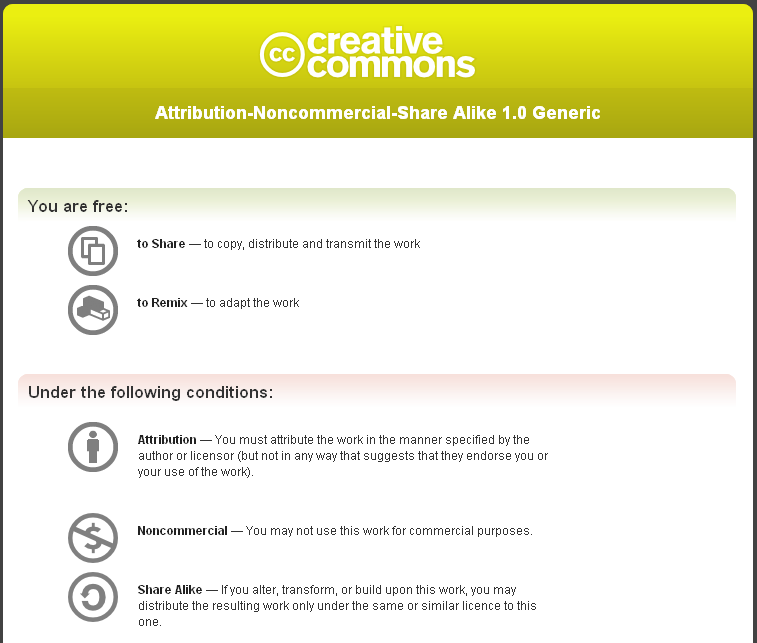
\includegraphics[width=0.50\textwidth]
		{pics/creative_common.png}
	\caption[Judul Gambar Tercetak di TOC]{Judul yang Tercetak di Halaman Ini.~\license. 
	{\small \emph{Sumber}: penulis.}}
	\label{fig:testGambar}
\end{figure}



%-----------------------------------------------------------------------------%
\section{Membuat Tabel}
%-----------------------------------------------------------------------------%
Seperti pada gambar, tabel juga dapat diberi label dan caption. 
Caption pada tabel terletak pada bagian atas tabel. 
Contoh tabel yang disarankan dapat dilihat pada \tab~\ref{tab:2-1}, \tab~\ref{tab:2-2} (format tabel dengan orientasi mendatar atau \emph{landscape}) dan \tab~\ref{tab:2-3} (format tabel untuk hasil pengujian statistik). Untuk penulisan tanda bintang (*) dalam tabel, dapat menggunakan perintah \texttt{\bslash sym\{***\}}. Sesuaikan jumlah bintang yang digunakan dengan tingkat signifikansi yang diinginkan.  

Tabel yang lebih dari satu halaman dapat dilihat di Lampiran \ref{apx:a}.
%\tab~\ref{tab:app1}.
Ada jenis tabel lain yang dapat dibuat dengan \latex~berikut 
beberapa diantaranya. 
Contoh-contoh ini bersumber dari 
\url{http://en.wikibooks.org/wiki/LaTeX/Tables}.

\begin{table}[htbp]
  \centering
  \caption{Peringkat Obligasi (Bentuk Tabel yang Disarankan)}\label{tab:2-1}
    \begin{tabular}{c p{.8\textwidth}}
\toprule
    Peringkat & \multicolumn{1}{c}{Keterangan} \\
\midrule
    AAA   & Peringkat tertinggi yang diberikan oleh PEFINDO. \textit{issuer} memiliki kapasitas untuk memenuhi kewajiban jangka panjang yang superior, relatif dengan \textit{issuer} lain di Indonesia. \\

    AA    & Hanya memiliki perbedaan yang kecil dengan peringkat tertinggi, \textit{issuer} memiliki kapasitas yang sangat kuat untuk memenuhi kewajiban jangka panjang, relatif dengan \textit{issuer} lain di Indonesia. \\

    A     & Memiliki kapasitas yang kuat dalam memenuhi kewajiban jangka panjang relatif dengan \textit{issuer} lain di Indonesia. Tetapi, \textit{issuer} lebih rentan terhadap perubahan situasi dan kondisi ekonomi yang merugikan dibandingkan dengan \textit{issuer} dengan peringkat lebih tinggi. \\

    BBB   & Memiliki kapasitas yang cukup untuk memenuhi kewajiban jangka panjang relatif dengan \textit{issuer} lain di Indonesia. Tetapi \textit{issuer} akan mengalami pelemahan kapasitas untuk memenuhi kewajiban apabila terjadi perubahan ekonomi dan situasi. \\

    BB    & Memiliki kapasitas yang agak lemah untuk memenuhi kawajiban jangka panjang relatif dengan \textit{issuer} lain di Indonesia. \textit{issuer} sedang menghadapi ketidakpastian atau kondisi bisnis, keuangan, atau ekonomi yang merugikan, yang mana dapat menyebabkan kurangnya kapasitas untuk memenuhi kewajiban. \\

    B     & Memiliki kapasitas yang lemah untuk memenuhi kewajiban jangka panjang relatif dengan \textit{issuer} lain di Indonesia. Kondisi bisnis, keuangan, atau ekonomi yang merugikan akan mengganggu kapasitas dan kemampuan \textit{issuer} untuk memenuhi kewajiban. \\

    CCC   & \textit{Issuer} dalam kondisi yang rentan dan keberlangsungan bergantung pada kondisi bisnis dan keuangan yang menguntungkan untuk memenuhi kewajiban. \\

    D/SD  & \textit{Issuer} gagal untuk memenuhi satu atau lebih dari kewajiban tepat waktu. SD (\textit{selective default}) merupakan peringkat yang diberikan PEFINDO ketika hanya obligasi tertentu saja yang mengalami kebangkrutan dan \textit{issuer} akan tetap melakukan pembayaran untuk obligasi lainnya. \\
    \bottomrule
\multicolumn{2}{l}{{\small \emph{Sumber}: PEFINDO.}}    
    \end{tabular}%
  \label{tab:addlabel}%
\end{table}%

\begin{sidewaystable}[p]
\centering
\caption{Korelasi Antar Variabel} \label{tab:2-2}
\begin{tabular}{l d{3}d{3}d{3}d{3}d{3}d{3}d{3}d{3}d{3}d{3}d{3}}
\toprule
 & \multicolumn{1}{c}{VAR1} &  \multicolumn{1}{c}{VAR2} &  \multicolumn{1}{c}{VAR3} &  \multicolumn{1}{c}{VAR4} &  \multicolumn{1}{c}{VAR5} &  \multicolumn{1}{c}{VAR6} &  \multicolumn{1}{c}{VAR7} &  \multicolumn{1}{c}{VAR8} &  \multicolumn{1}{c}{VAR9} &  \multicolumn{1}{c}{VAR10} & \multicolumn{1}{c}{VAR11} \\
\midrule
VAR1 & 1 \\
VAR2 & -0,255 & 1 \\
VAR3 & -0,004 & -0,195 & 1 \\
VAR4 & 0,223 & -0,062 & 0,672 & 1 \\
VAR5 & 0,026 & 0,102 & 0,393 & -0,194 & 1 \\
VAR6 & 0,038 & 0,127 & 0,174 & -0,104 & -0,187 & 1 \\
VAR7 & 0,192 & 0,135 & 0,021 & -0,062 & -0,063 & 0,101 & 1 \\
VAR8 & 0,265 & 0,168 & -0,024 & -0,06 & -0,049 & 0,072 & 0,001 & 1 \\
VAR9 & 0,275 & 0,366 & -0,108 & 0,091 & 0,954 & -0,087 & -0,033 & 0,313 & 1 \\
VAR10 & 0,786 & 0,322 & -0,117 & 0,316 & -0,098 & -0,295 & 0,278 & 0,023 & 0,316 & 1 \\
VAR11 & 0,275 & 0,316 & -0,108 & 0,054 & -0,087 & -0,033 & 0,021 & -0,062 & -0,063 & 0,023 & 1 \\
\bottomrule
\multicolumn{12}{p{.5\textwidth}}{\footnotesize \emph{Sumber}: olahan penulis.}
\end{tabular}
\end{sidewaystable}


\begin{table}[htbp]
  \centering
  \caption{Hasil Pemodelan (Sebuah Ilustrasi)}\label{tab:2-3}
  	\begin{tabular}{l d{3} d{3} c d{3} d{3} @{\hspace{5pt}}} 
	\toprule
& \multicolumn{4}{c}{Variabel terikat: Investasi} \\ \cmidrule{2-6}	
& \multicolumn{2}{c}{OLS} &  & \multicolumn{2}{c}{GMM} \\ \cmidrule{2-3}\cmidrule{5-6}
& \multicolumn{1}{c}{(1)} 	& \multicolumn{1}{c}{(2)} 	&& \multicolumn{1}{c}{(3)} & \multicolumn{1}{c}{(4)}\\
 \midrule
Pendapatan			& 0,114\sym{**} 	& 0,0535\sym{*} 	&& 0,455\sym{***}  & 0,202\sym{*}  \\
					&(0,0078) 			& (0,089) 		&& (0,024) 	& (0,066) 		\\ 
\midrule
	Perusahaan 		& 3014     			&  3014			&& 2946 	& 2946   \\
	Observasi 		& 15070     			& 15070 			&&  14730	& 14730 \\
    \emph{Firm-year fixed effect} &	\multicolumn{1}{c}{Tidak}    & \multicolumn{1}{c}{Ya}   &&	\multicolumn{1}{c}{Tidak}    	& \multicolumn{1}{c}{Ya} \\
    \emph{Arellano-Bond statistic} 		&	&	&& 18,29 	& 19,294\\
    \emph{p-value}					&	&	&& 0,010	& 0,087 \\
    $R^2$  			& 0,090 	& 0,236 	&& -0,324 & 0,185 \\
    \bottomrule
    \multicolumn{6}{p{.95\textwidth}}{\textit{Keterangan}: \sym{*} signifikan pada tingkat 1\%,
     \sym{**} signifikan pada tingkat 5\%,\sym{***} signifikan pada tingkat 10\%. 
     (1) menunjukkan estimasi model dengan persamaan \eqref{eq:gabungan1}, (2) menunjukkan estimasi model dengan persamaan \eqref{eq:gabungan2}. Angka di dalam tanda kurung menunjukkan \textit{standard error}. }\\
         \multicolumn{6}{p{.95\textwidth}}{{\small \emph{Sumber}: olahan penulis.}} 
    \end{tabular}
\end{table}

%-----------------------------------------------------------------------------%
\section{Satu Persamaan}
%-----------------------------------------------------------------------------%
\begin{equation}\label{eq:garis}
	\cfrac{y - y_{1}}{y_{2} - y_{1}} = 
	\cfrac{x - x_{1}}{x_{2} - x_{1}}
\end{equation}

\equ~\eqref{eq:garis} di atas adalah persamaan garis. 
\equ~\eqref{eq:garis} dibuat dengan perintah \bslash \texttt{equation}
dan dan \eqref{eq:bola} dibuat dengan perintah \bslash \texttt{align}. 
\begin{equation}\label{eq:bola}
	\underbrace{|\overline{ab}|}_{\text{pada bola $|\overline{ab}| = r$}} 
		= \sqrt[2]{(x_{b} - x_{a})^{2} + (y_{b} - y_{a})^{2} + 
				\vert\vert(z_{b} - z_{a})^{2}}.
\end{equation}

%-----------------------------------------------------------------------------%
\section{Lebih dari Satu Persamaan}
\label{sec:multiEqu}
%-----------------------------------------------------------------------------%
Untuk menulis persamaan lebih dari satu baris, kita dapat menggunakan perintah \bslash \texttt{equation} 
dan \bslash \texttt{split} sebagai berikut:
\begin{equation}\label{eq:matriks1}	
\begin{split}
	|\overline{a} \times \overline{b}| &= |\overline{a}| |\overline{b}| \sin\theta 
		\\[0.2cm]
	\overline{a} \times \overline{b} &=  
		\begin{array}{| c c c |}
			\hat{i} & x_{1} & x_{2} \\
			\hat{j} & y_{1} & y_{2} \\
			\hat{k} & z_{1} & z_{2} \\
		\end{array}  \\[0.2cm]
	&= \hat{i} \,
		\begin{array}{ | c c | }
			y_{1} & y_{2} \\
			z_{1} & z_{2} \\
		\end{array} 
	   + \hat{j} \,
		\begin{array}{ | c c | }
			z_{1} & z_{2} \\
			x_{1} & x_{2} \\
		\end{array} 
	   + \hat{k} \,	
		\begin{array}{ | c c | }
			x_{1} & x_{2} \\
			y_{1} & y_{2} \\
		\end{array}.
\end{split}
\end{equation}

\equ~\eqref{eq:matriks1} juga dapat ditulis menggunakan  perintah \bslash \texttt{align} sebagai berikut: 
\begin{align}\label{eq:matriks2}	
	|\overline{a} \times \overline{b}| &= |\overline{a}| |\overline{b}| \sin\theta \nonumber
		\\[0.2cm]
	\overline{a} \times \overline{b} &=  
		\begin{array}{| c c c |}
			\hat{i} & x_{1} & x_{2} \\
			\hat{j} & y_{1} & y_{2} \\
			\hat{k} & z_{1} & z_{2} \\
		\end{array}  \\[0.2cm]
	&= \hat{i} \,
		\begin{array}{ | c c | }
			y_{1} & y_{2} \\
			z_{1} & z_{2} \\
		\end{array} 
	   + \hat{j} \,
		\begin{array}{ | c c | }
			z_{1} & z_{2} \\
			x_{1} & x_{2} \\
		\end{array} 
	   + \hat{k} \,	
		\begin{array}{ | c c | }
			x_{1} & x_{2} \\
			y_{1} & y_{2} \\
		\end{array}.
		\nonumber
\end{align}
Pada \equ~\eqref{eq:matriks2} dapat dilihat beberapa baris menjadi satu bagian 
dari \equ~\eqref{eq:matriks2}. 

Perbedaan antara \equ~\eqref{eq:matriks1} dan \equ~\eqref{eq:matriks2} adalah pada \equ~\eqref{eq:matriks1}, 
kita tidak perlu menulis \bslash\texttt{nonumber} di setiap baris persamaan. 
Untuk menghilangkan penomoran rumus di seluruh baris di  \equ~\eqref{eq:matriks1}, kita menggunakan perintah 
\bslash \texttt{begin\{equation*\}} dan \bslash \texttt{end\{equation*\}}.  

Sedangkan di bawah ini dapat dilihat bahwa dengan cara menggunakan perintah  \bslash \texttt{align},
 \equ~\eqref{eq:gabungan1}, \eqref{eq:gabungan2}, dan \eqref{eq:gabungan3} memiliki nomor 
persamaannya masing-masing. 

\noindent \begin{align}\label{eq:gabungan1}	
	\int_{a}^{b} f(x)\, dx + \int_{b}^{c} f(x) \, dx = \int_{a}^{c} f(x) \, dx
		\\\label{eq:gabungan2}
	\lim_{x \to \infty} \frac{f(x)}{g(x)} = 0 \hspace{1cm} 
		\text{jika pangkat $f(x)$ $<$ pangkat $g(x)$} \\\label{eq:gabungan3}
	a^{m^{a \, ^{n}\log b }} = b^{\frac{m}{n}}
\end{align}

Contoh penulisan matriks dapat dilihat di \equ~\eqref{eq:matrix}.

\begin{equation}
A_{m,n} = 
 \begin{pmatrix}
  a_{1,1} & a_{1,2} & \cdots & a_{1,n} \\
  a_{2,1} & a_{2,2} & \cdots & a_{2,n} \\
  \vdots  & \vdots  & \ddots & \vdots  \\
  a_{m,1} & a_{m,2} & \cdots & a_{m,n} 
 \end{pmatrix}
 \label{eq:matrix}
\end{equation}
%-----------------------------------------------------------------------------%
\section{Penulisan rumus yang panjang}
\label{sec:longEqu}
%-----------------------------------------------------------------------------%
Penulisan rumus yang panjang sebagai berikut:
\begin{equation}
\begin{split}
\textit{OZIndex}_t =& -3,002 \times \textit{CashFlow}_t + 0,483 \times Q_t + 
3,139 \times \textit{Leverage}_t   \\
	& -30,368 \times \textit{Dividends}_t - 3,315 \times \textit{CashHoldings}_t
\end{split}
\label{eq:3-1}
\end{equation}
dengan 

\begin{tabular}{l@{~:~}l}
\textit{OZIndex}$_t$ & indeks OZ \\
\textit{Q}$_t$ & Tobin's q pada tahun $t$ \\
\textit{CashFlow}$_t$ & arus kas perusahaan pada tahun $t$ \\
\textit{Leverage}$_t$ & jumlah utang perusahaan pada tahun $t$ \\
\textit{Dividends}$_t$ & jumlah dividen yang dibayarkan pada akhir tahun $t$ \\
\textit{CashHoldings}$_t$ & jumlah kas yang dimiliki pada tahun $t$. \\
\end{tabular}\\

\noindent Penulisan matematika lebih lanjut dapat dibaca di \url{https://en.wikibooks.org/wiki/LaTeX/Mathematics}.
TEST

%-----------------------------------------------------------------------------%
\section{Huruf Yunani (\textit{Greek Letters})}
\label{sec:greek}
%-----------------------------------------------------------------------------%
\begin{table}[htbp]
\centering
\begin{tabular}{|c|c|} \hline
\( \begin{array}{cl}
\alpha & \verb+\alpha+ \\
\beta & \verb+\beta+ \\
\gamma & \verb+\gamma+ \\
\delta & \verb+\delta+ \\
\lambda & \verb+\lambda+ \\
\omega & \verb+\omega+ \\
\psi & \verb+\psi+ \\
\chi & \verb+\chi+ \\
\rho  & \verb+\rho + \\
\epsilon & \verb+\epsilon+ \\
\kappa & \verb+\kappa+ \\
\pi & \verb+\pi+ \\
\phi & \verb+\phi+ \\
\sigma & \verb+\sigma+ \\
\theta & \verb+\theta+ \\
\end{array} \)
&
\( \begin{array}{cl}
\upsilon & \verb+\upsilon+ \\
\xi & \verb+\xi+ \\
\tau & \verb+\tau+ \\
\iota & \verb+\iota+ \\
\eta & \verb+\eta+ \\
\zeta & \verb+\zeta+ \\
\mu& \verb+\mu+ \\
\nu & \verb+\nu+ \\
\varrho & \verb+\varrho+ \\
\varepsilon & \verb+\varepsilon+ \\
\varpi & \verb+\varpi+ \\
\varphi & \verb+\varphi+ \\
\varsigma & \verb+\varsigma+ \\
\vartheta & \verb+\vartheta+ 
\end{array} \)
\\ \hline
\end{tabular}
\end{table}

\begin{table}[htbp]
\centering
\begin{tabular}{|c|c|} \hline
\( \begin{array}{cl}
\Gamma & \verb+\Gamma+ \\
\Delta & \verb+\Delta+ \\
\Lambda & \verb+\Lambda+ \\
\Omega & \verb+\Omega+ \\
\Pi & \verb+\Pi+ \\
\Phi & \verb+\Phi+ \\
\Psi & \verb+\Psi+ \\
\Sigma & \verb+\Sigma+ \\
\Theta & \verb+\Theta+ \\
\Upsilon & \verb+\Upsilon+ \\
\Xi & \verb+\Xi+ \\
\end{array} \)
&
\( \begin{array}{cl}
\varGamma & \verb+\varGamma+ \\
\varDelta & \verb+\varDelta+ \\
\varLambda & \verb+\varLambda+ \\
\varOmega & \verb+\varOmega+ \\
\varPi & \verb+\varPi+ \\
\varPhi & \verb+\varPhi+ \\
\varPsi & \verb+\varPsi+ \\
\varSigma & \verb+\varSigma+ \\
\varTheta & \verb+\varTheta+ \\
\varUpsilon & \verb+\varUpsilon+ \\
\varXi & \verb+\varXi+ \\
\aleph & \verb+\aleph+
\end{array} \)
\\ \hline

\end{tabular}
\end{table}


%-----------------------------------------------------------------------------%
\section{Simbol Umum Lainnya}
\label{sec:sym}
%-----------------------------------------------------------------------------%


\begin{table}[htbp]
\centering
\begin{tabular}{|c|c|c|} \hline
\( \begin{array}{cl}
\neq & \verb+\neq+ \\
\approx & \verb+\approx+ \\
\equiv & \verb+\equiv+ \\
\cong & \verb+\cong+ \\
\simeq & \verb+\simeq+ \\
\partial & \verb+\partial+ \\
\infty & \verb+\infty+ \\
\nabla & \verb+\nabla+ \\
\exists & \verb+\exists+ \\
\ell & \verb+\ell+ \\
\vee & \verb+\vee+ \\
\wedge & \verb+\wedge+ \\
\forall & \verb+\forall+ 
\end{array} \)
&
\( \begin{array}{cl}
\pm  &\verb+\pm+ \\
\mp  &\verb+\mp+ \\
\times &\verb+\times+ \\
\div &\verb+\div+ \\
\cup & \verb+\cup+ \\
\cap & \verb+\cap+ \\
\in & \verb+\in+ \\
\notin & \verb+\notin+ \\
\setminus & \verb+\setminus+\\ 
\subset & \verb+\subset+ \\
\supset & \verb+\supset+ \\
\cdot & \verb+\cdot+ \\
\copyright & \verb+\copyright+ 
\end{array} \)
&
\( \begin{array}{cl}
\to & \verb+\to+ \\
\iff & \verb+\iff+ \\
\$ & \verb+\$+ \\
\pounds & \verb+\pounds+ \\
\% & \verb+\%+ \\
\& & \verb+\&+ \\
\{ & \verb+\{+ \\
\} & \verb+\}+ \\
\_ & \verb+\_+ \\
\P & \verb+\P+ \\
\S  & \verb+\S + \\
\ast & \verb+\ast+ \\
\dag & \verb+\dag+ \\
\ddag & \verb+\ddag+ \\
\bullet & \verb+\bullet+
\end{array} \)
\\ \hline
\end{tabular}
\end{table}
